% F049: native TikZ/PGFPlots, computed from the stated mathematical model.
\begin{center}
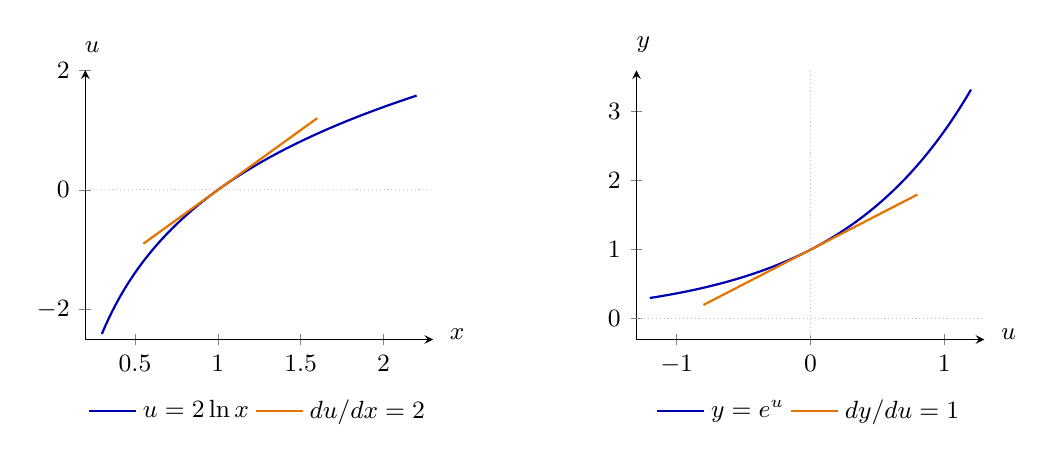
\begin{tikzpicture}[font=\small,>=stealth]
\begin{axis}[width=6cm,height=5cm,xmin=0.2,xmax=2.3,ymin=-2.5,ymax=2,
axis lines=left,xlabel={$x$},ylabel={$y$},font=\small,
xlabel style={at={(axis description cs:1.02,.02)},anchor=west},
ylabel style={rotate=-90,at={(axis description cs:.02,1.03)},anchor=south},
legend style={at={(axis description cs:.5,-.18)},anchor=north,draw=none,fill=none,font=\small,legend columns=2},
unbounded coords=jump,clip=true,at={(0,0)},anchor=south west,ylabel={$u$}]
\addplot[gray!45,thin,densely dotted,forget plot] coordinates {(0.2,0) (2.3,0)};
\addplot[blue!70!black,thick] coordinates {(0.3,-2.4079456) (0.31055556,-2.3387849) (0.32111111,-2.2719362) (0.33166667,-2.2072497) (0.34222222,-2.14459) (0.35277778,-2.0838339) (0.36333333,-2.0248692) (0.37388889,-1.9675932) (0.38444444,-1.911912) (0.395,-1.857739) (0.40555556,-1.8049948) (0.41611111,-1.7536059) (0.42666667,-1.7035044) (0.43722222,-1.6546274) (0.44777778,-1.6069164) (0.45833333,-1.5603171) (0.46888889,-1.5147789) (0.47944444,-1.4702545) (0.49,-1.4266998) (0.50055556,-1.3840734) (0.51111111,-1.3423365) (0.52166667,-1.3014529) (0.53222222,-1.2613883) (0.54277778,-1.2221106) (0.55333333,-1.1835894) (0.56388889,-1.1457961) (0.57444444,-1.1087038) (0.585,-1.0722869) (0.59555556,-1.0365212) (0.60611111,-1.0013839) (0.61666667,-0.9668533) (0.62722222,-0.93290876) (0.63777778,-0.89953073) (0.64833333,-0.86670062) (0.65888889,-0.83440073) (0.66944444,-0.8026142) (0.68,-0.77132496) (0.69055556,-0.7405177) (0.70111111,-0.7101778) (0.71166667,-0.68029128) (0.72222222,-0.6508448) (0.73277778,-0.62182558) (0.74333333,-0.59322141) (0.75388889,-0.56502057) (0.76444444,-0.53721185) (0.775,-0.5097845) (0.78555556,-0.48272819) (0.79611111,-0.45603303) (0.80666667,-0.4296895) (0.81722222,-0.40368845) (0.82777778,-0.37802109) (0.83833333,-0.35267897) (0.84888889,-0.32765395) (0.85944444,-0.30293819) (0.87,-0.27852413) (0.88055556,-0.25440452) (0.89111111,-0.23057231) (0.90166667,-0.20702075) (0.91222222,-0.18374331) (0.92277778,-0.16073367) (0.93333333,-0.13798574) (0.94388889,-0.11549364) (0.95444444,-0.093251683) (0.965,-0.071254355) (0.97555556,-0.049496339) (0.98611111,-0.027972484) (0.99666667,-0.0066778025) (1.0072222,0.014392534) (1.0177778,0.035243203) (1.0283333,0.055878737) (1.0388889,0.076303532) (1.0494444,0.096521847) (1.06,0.11653782) (1.0705556,0.13635545) (1.0811111,0.15597864) (1.0916667,0.17541116) (1.1022222,0.19465669) (1.1127778,0.21371878) (1.1233333,0.23260091) (1.1338889,0.25130644) (1.1444444,0.26983864) (1.155,0.28820069) (1.1655556,0.30639569) (1.1761111,0.32442665) (1.1866667,0.34229651) (1.1972222,0.36000812) (1.2077778,0.37756425) (1.2183333,0.39496761) (1.2288889,0.41222084) (1.2394444,0.4293265) (1.25,0.4462871) (1.2605556,0.46310508) (1.2711111,0.47978282) (1.2816667,0.49632263) (1.2922222,0.51272678) (1.3027778,0.52899747) (1.3133333,0.54513687) (1.3238889,0.56114707) (1.3344444,0.57703012) (1.345,0.59278803) (1.3555556,0.60842275) (1.3661111,0.6239362) (1.3766667,0.63933024) (1.3872222,0.65460669) (1.3977778,0.66976735) (1.4083333,0.68481394) (1.4188889,0.69974819) (1.4294444,0.71457174) (1.44,0.72928623) (1.4505556,0.74389325) (1.4611111,0.75839436) (1.4716667,0.77279109) (1.4822222,0.78708493) (1.4927778,0.80127733) (1.5033333,0.81536973) (1.5138889,0.82936353) (1.5244444,0.84326009) (1.535,0.85706076) (1.5455556,0.87076686) (1.5561111,0.88437966) (1.5666667,0.89790044) (1.5772222,0.91133043) (1.5877778,0.92467083) (1.5983333,0.93792284) (1.6088889,0.95108762) (1.6194444,0.96416631) (1.63,0.97716003) (1.6405556,0.99006988) (1.6511111,1.0028969) (1.6616667,1.0156422) (1.6722222,1.0283068) (1.6827778,1.0408917) (1.6933333,1.0533979) (1.7038889,1.0658264) (1.7144444,1.0781782) (1.725,1.0904541) (1.7355556,1.1026551) (1.7461111,1.1147822) (1.7566667,1.1268361) (1.7672222,1.1388179) (1.7777778,1.1507283) (1.7883333,1.1625682) (1.7988889,1.1743384) (1.8094444,1.1860397) (1.82,1.197673) (1.8305556,1.209239) (1.8411111,1.2207385) (1.8516667,1.2321723) (1.8622222,1.243541) (1.8727778,1.2548455) (1.8833333,1.2660865) (1.8938889,1.2772647) (1.9044444,1.2883807) (1.915,1.2994352) (1.9255556,1.3104291) (1.9361111,1.3213628) (1.9466667,1.332237) (1.9572222,1.3430525) (1.9677778,1.3538097) (1.9783333,1.3645095) (1.9888889,1.3751523) (1.9994444,1.3857387) (2.01,1.3962694) (2.0205556,1.406745) (2.0311111,1.417166) (2.0416667,1.4275329) (2.0522222,1.4378464) (2.0627778,1.448107) (2.0733333,1.4583152) (2.0838889,1.4684716) (2.0944444,1.4785767) (2.105,1.4886309) (2.1155556,1.4986349) (2.1261111,1.5085891) (2.1366667,1.518494) (2.1472222,1.52835) (2.1577778,1.5381578) (2.1683333,1.5479176) (2.1788889,1.5576301) (2.1894444,1.5672957) (2.2,1.5769147)};
\addlegendentry{$u=2\ln x$}
\addplot[orange!90!black,thick] coordinates {(0.55,-0.9) (1.6,1.2)};
\addlegendentry{$du/dx=2$}
\end{axis}\begin{axis}[width=6cm,height=5cm,xmin=-1.3,xmax=1.3,ymin=-0.3,ymax=3.6,
axis lines=left,xlabel={$x$},ylabel={$y$},font=\small,
xlabel style={at={(axis description cs:1.02,.02)},anchor=west},
ylabel style={rotate=-90,at={(axis description cs:.02,1.03)},anchor=south},
legend style={at={(axis description cs:.5,-.18)},anchor=north,draw=none,fill=none,font=\small,legend columns=2},
unbounded coords=jump,clip=true,at={(7cm,0)},anchor=south west,xlabel={$u$}]
\addplot[gray!45,thin,densely dotted,forget plot] coordinates {(-1.3,0) (1.3,0)};
\addplot[gray!45,thin,densely dotted,forget plot] coordinates {(0,-0.3) (0,3.6)};
\addplot[blue!70!black,thick] coordinates {(-1.2,0.30119421) (-1.1866667,0.30523703) (-1.1733333,0.30933411) (-1.16,0.31348618) (-1.1466667,0.31769399) (-1.1333333,0.32195827) (-1.12,0.32627979) (-1.1066667,0.33065932) (-1.0933333,0.33509764) (-1.08,0.33959553) (-1.0666667,0.34415379) (-1.0533333,0.34877323) (-1.04,0.35345468) (-1.0266667,0.35819897) (-1.0133333,0.36300694) (-1,0.36787944) (-0.98666667,0.37281735) (-0.97333333,0.37782153) (-0.96,0.38289289) (-0.94666667,0.38803231) (-0.93333333,0.39324072) (-0.92,0.39851904) (-0.90666667,0.40386821) (-0.89333333,0.40928918) (-0.88,0.41478291) (-0.86666667,0.42035038) (-0.85333333,0.42599259) (-0.84,0.43171052) (-0.82666667,0.43750521) (-0.81333333,0.44337767) (-0.8,0.44932896) (-0.78666667,0.45536014) (-0.77333333,0.46147226) (-0.76,0.46766643) (-0.74666667,0.47394374) (-0.73333333,0.4803053) (-0.72,0.48675226) (-0.70666667,0.49328575) (-0.69333333,0.49990693) (-0.68,0.50661699) (-0.66666667,0.51341712) (-0.65333333,0.52030852) (-0.64,0.52729242) (-0.62666667,0.53437007) (-0.61333333,0.54154271) (-0.6,0.54881164) (-0.58666667,0.55617813) (-0.57333333,0.56364349) (-0.56,0.57120906) (-0.54666667,0.57887619) (-0.53333333,0.58664622) (-0.52,0.59452055) (-0.50666667,0.60250057) (-0.49333333,0.61058771) (-0.48,0.61878339) (-0.46666667,0.62708909) (-0.45333333,0.63550626) (-0.44,0.64403642) (-0.42666667,0.65268108) (-0.41333333,0.66144177) (-0.4,0.67032005) (-0.38666667,0.6793175) (-0.37333333,0.68843572) (-0.36,0.69767633) (-0.34666667,0.70704097) (-0.33333333,0.71653131) (-0.32,0.72614904) (-0.30666667,0.73589586) (-0.29333333,0.74577351) (-0.28,0.75578374) (-0.26666667,0.76592834) (-0.25333333,0.7762091) (-0.24,0.78662786) (-0.22666667,0.79718647) (-0.21333333,0.8078868) (-0.2,0.81873075) (-0.18666667,0.82972026) (-0.17333333,0.84085728) (-0.16,0.85214379) (-0.14666667,0.86358179) (-0.13333333,0.87517332) (-0.12,0.88692044) (-0.10666667,0.89882523) (-0.093333333,0.91088982) (-0.08,0.92311635) (-0.066666667,0.93550699) (-0.053333333,0.94806394) (-0.04,0.96078944) (-0.026666667,0.97368575) (-0.013333333,0.98675516) (0,1) (0.013333333,1.0134226) (0.026666667,1.0270254) (0.04,1.0408108) (0.053333333,1.0547812) (0.066666667,1.0689391) (0.08,1.0832871) (0.093333333,1.0978276) (0.10666667,1.1125633) (0.12,1.1274969) (0.13333333,1.1426308) (0.14666667,1.1579679) (0.16,1.1735109) (0.17333333,1.1892625) (0.18666667,1.2052255) (0.2,1.2214028) (0.21333333,1.2377972) (0.22666667,1.2544117) (0.24,1.2712492) (0.25333333,1.2883126) (0.26666667,1.3056052) (0.28,1.3231298) (0.29333333,1.3408897) (0.30666667,1.3588879) (0.32,1.3771278) (0.33333333,1.3956124) (0.34666667,1.4143452) (0.36,1.4333294) (0.37333333,1.4525684) (0.38666667,1.4720657) (0.4,1.4918247) (0.41333333,1.5118489) (0.42666667,1.5321419) (0.44,1.5527072) (0.45333333,1.5735486) (0.46666667,1.5946698) (0.48,1.6160744) (0.49333333,1.6377664) (0.50666667,1.6597495) (0.52,1.6820276) (0.53333333,1.7046049) (0.54666667,1.7274851) (0.56,1.7506725) (0.57333333,1.7741711) (0.58666667,1.7979851) (0.6,1.8221188) (0.61333333,1.8465764) (0.62666667,1.8713623) (0.64,1.8964809) (0.65333333,1.9219366) (0.66666667,1.947734) (0.68,1.9738777) (0.69333333,2.0003723) (0.70666667,2.0272226) (0.72,2.0544332) (0.73333333,2.0820091) (0.74666667,2.1099551) (0.76,2.1382762) (0.77333333,2.1669775) (0.78666667,2.196064) (0.8,2.2255409) (0.81333333,2.2554135) (0.82666667,2.2856871) (0.84,2.316367) (0.85333333,2.3474587) (0.86666667,2.3789677) (0.88,2.4108997) (0.89333333,2.4432603) (0.90666667,2.4760552) (0.92,2.5092904) (0.93333333,2.5429716) (0.94666667,2.577105) (0.96,2.6116965) (0.97333333,2.6467523) (0.98666667,2.6822786) (1,2.7182818) (1.0133333,2.7547683) (1.0266667,2.7917445) (1.04,2.829217) (1.0533333,2.8671925) (1.0666667,2.9056777) (1.08,2.9446796) (1.0933333,2.9842049) (1.1066667,3.0242607) (1.12,3.0648542) (1.1333333,3.1059926) (1.1466667,3.1476831) (1.16,3.1899333) (1.1733333,3.2327505) (1.1866667,3.2761425) (1.2,3.3201169)};
\addlegendentry{$y=e^u$}
\addplot[orange!90!black,thick] coordinates {(-0.8,0.2) (0.8,1.8)};
\addlegendentry{$dy/du=1$}
\end{axis}
\end{tikzpicture}
\par\smallskip{\small 在 $x=1,u=0$ 处，合成函数 $y=x^2$ 的斜率为 $2\times1=2$。左图自变量为 $x$，右图自变量为 $u$。}
\end{center}
